\section{Project 9 - Image Segmentation}

\subsection{Project Proposal}
There tow parts of project 9. One task is for edge detection: implement the Roberts, Prewitt, Sobel, the Marr-Hildreth and the Canny edge detectors. The test image is \emph{building.tif}. The other task is to implement the Otsu’s method of thresholding segmentation, and compare the results with the global thresholding method using test image \emph{polymersomes.tif}.

\subsection{Preliminaries}
\subsubsection{Edge detection}
The central idea of edge detection is that local changes in intensity can be detected using derivatives. We have the following conclusions which show that first- and second-order derivatives are particularly well suited for this purpose: (1) First-order derivatives generally produce thicker edges in an image. (2) Second-order derivatives have a stronger response to fine details such as thin lines, isolated points, and noise. (3) Second-order derivatives produce a double-edge response at ramp and step transitions in intensity. (4) The sign of the second derivative can be used to determine whether a transition into an edge is from light to dark or dark to light.

\subsubsection{Basic edge detection}
The tool of choice for finding edge strength and direction at location $(x, y)$ of an image $f$ is the gradient. 
\begin{equation} \nabla f \equiv \text{grad}(f) \equiv \left[ \begin{array}{c} g_x \\ g_y \end{array}\right] = \left[ \begin{array}{c} \frac{\partial f}{\partial x} \\ \frac{\partial f}{\partial y} \end{array} \right] 
\end{equation}
The magnitude of vector $\nabla f$ defined as \begin{equation} \label{eq:magnitude} M(x,y)=mag(\nabla f) =  \sqrt{g_x^2 + g_y^2} \approx |g_x| + |g_y| \end{equation} is the value of the rate of change in the direction of the gradient vector. The second $=$ is a frequently used approximate to avoid square roots. The direction of gradient vector is given by the angle \begin{equation} \alpha(x,y)=\tan^{-1} \left[ \frac{g_y}{g_x} \right] \label{eq:angle} \end{equation}
The direction of an edge at an arbitrary point $(x,y)$ is orthogonal to the direction $\alpha(x,y)$. 
Here we mention three masks(Figure \ref{fig:3masks}) Roberts, Prewitt and Sobel which can be used to compute the gradient of the center point with convolution operation.
\begin{figure}[h!]
	\centering
	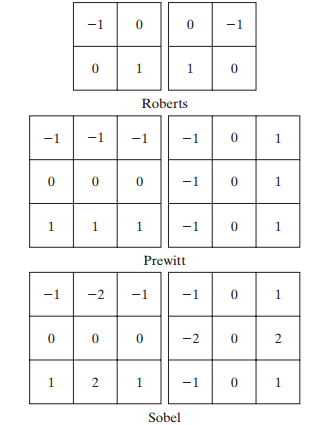
\includegraphics[scale=0.7]{myfigure/p9/3masks.png}
	\caption{3 masks for gradient computation: Roberts, Prewitt, Sobel}
	\label{fig:3masks}
\end{figure}

\subsubsection{More advanced techniques for edge detection}
\textbf{The Marr-Hildreth edge detector} is able to compute the approximate numerical result of gradient operator for sharply focused detail as well as act at large scale to detect the blurry edges. This operator is defined as $\nabla^2 G$ where \begin{equation}G(x,y) = e^{-frac{x^2+y^2}{2\sigma^2}} \label{eq:gaussian_2}\end{equation}. Then the so-called \emph{Laplacian of Gaussian(LoG)} is \begin{equation} \nabla^2 G(x,y) = \left[ \frac{x^2+y^2-\sigma^2}{4\sigma^4} \right]e^{-\frac{x^2+y^2}{2\sigma^2}} \end{equation} The use of LoG filter can be represented as \begin{equation} g(x,y)=\nabla^2\left[G(x,y)\right]\circ f(x,y) \end{equation}. Because of linear process, we can also write it as \begin{equation} g(x,y)=\nabla^2\left[G(x,y)\circ f(x,y)\right] \end{equation} 
Hence, the steps of Marr-Hildreth algorithm can be summarized as: \textbf{1.}Filter the input image with $n\times n$ Gaussian lowpass filter obtained by sampling \ref{eq:gaussian_2}. \textbf{2.}Compute the Laplacian of the result of step \textbf{1} using, for example, $3\times 3$ mask. \textbf{3.}Find the zero crossing of the resulting image from step 2. \\
The method of finding zero crossing at any pixel $p$ is to use a $3\times 3$ neighborhood centered at $p$, if the absolute difference of any two opposite neighbors exceeds a given threshold, then $p$ is a zero-crossing pixel.\\
\textbf{The Canny edge detector} is superior in general to all the detectors discussed before. The algorithm consist the following steps: \\
\textbf{1.}Smooth the input image with a Gaussian filter.\\ 
\textbf{2.}Compute the gradient magnitude $M(x,y)$ and angle $\alpha(x,y)$ images. \\
\textbf{3.}Apply nonmaxima suppression to the gradient magnitude image. \\
\textbf{4.}Use double thresholding and connectivity analysis to detect and link edge. \\
The first two steps are apparent as the definition in Eq.\ref{eq:magnitude} and Eq.\ref{eq:angle}. The step \textbf{3 nonmaxima suppression} is used to thin the coarse edges in magnitude image. The essence of nonmaxima suppression is to define a set of discrete orientation of the edge normal $\{ d_1, d_2, d_3, d_4 \}$, e.g. $0^\circ$, $45^\circ$, $90^\circ$, $-45^\circ$. To map edges of arbitrary direction to the discrete orientation, we define non-overlapping range for each given direction. We can formulate the nonmaxima suppression schema for a $3\times 3$ region centered at every point $(x,y)$ in angle image $\alpha(x,y)$: \\
\textbf{(1)}Find the direction $d_k$ that is closest to $\alpha(x,y)$. \\
\textbf{(2)}If the value of $M(x,y)$ is less than at least one of its two neighbor on this direction, let $g_N(x,y)=0$; otherwise, let $g_N(x,y)=M(x,y)$. \\
Then we come to step \textbf{4 double thresholding} on $g_N(x,y)$ to reduce the false edge points. In Canny's algorithm we use two thresholds, $T_L$ as the low threshold and $T_H$ as the high threshold. Canny suggests that the ratio of the high to low threshold should be two or three to one. The process of thresholding is, \begin{equation} g_{NH}(x,y)=g_N(x,y)\geq T_H \end{equation}\begin{equation} g_{NL}(x,y)=g_N(x,y)\geq T_L\end{equation} then eliminate all the nonzero pixels in $g_{NH}$ from $g_{NL}$ \begin{equation} g_{NL}(x,y) := g_{NL}(x,y)-g_{NH}(x,y) \end{equation} The pixels in $g_{NH}$ is viewed as strong valid edge pixels and are marked immediately, but there are many gaps on these edges that should be filled using information from $g_{NL}$. We do this by following these steps:\\
\textbf{(1)}Locate the next unvisited edge pixel $p$ in $g_{NH}$. \\
\textbf{(2)}Mark all the weak pixels in $g_{NL}$ that is 8-connective to $p$ as valid. \\
\textbf{(3)}If all nonzero pixels in $g_{NH}$ has been visited, goto step 4. Otherwise goto back to step 1. \\
\textbf{(4)}Set all the pixels that are not marked as valid in $g_{NL}$.\\
The final result of Canny's algorithm is formed by appending all the nonzero pixels in $g_{NL}$ to $g_{NH}$.
\subsubsection{Thresholding Segmentation}
Thresholding is useful in applications of image segmentation because of its simplicity of implementation and computational speed. We talk about the most basic intensity thresholding here. The basic formula is 
\begin{equation}g(x,y)=\left \{ \begin{array}{rcl}
1 & \text{if}f(x,y)>T \\
0 & \text{otherwise}  \end{array} \right.\label{eq:global_threshold}\end{equation}
When $T$ is a constant applicable over an entire image, the process given in this equation is referred to as \textbf{global thresholding}. \\
\textbf{Basic global thresholding} algorithm is capable of estimate automatically the threshold value for each image is required. The following iterative algorithm can be used for this purpose:\\
\textbf{1.}Select an initial estimate for the global threshold $T$. Mean value of gray intensities is a good choice.\\
\textbf{2.}Segment the image using $T$ in Eq.\ref{eq:global_threshold}. This will result in two groups of pixels: $G_1$($g(x,y)>T$) and $G_2$($g(x,y)\leq T$)\\
\textbf{3.}Compute the average intensity values $m_1$ and $m_2$ for the two groups $G_1$ and $G_2$ respectively.\\
\textbf{4.}Compute a new threshold value: $T=(m_1+m_2)/2$\\
\textbf{5.}Repeat step2 through 4 until the difference between values of $T$ in successive iterations os smaller than a predefined parameter $\Delta T$.\\
Global thresholding seems very simple as we just need to select a proper value for $T$, but the problem is that, usually, we cannot directly find out such a $T$ that separates the hills in histogram. Noise in the image, illumination and reflectance and so on factors lead to this effect.
Then we discuss an attractive alternative \textbf{Otus's method} which is based entirely on computations performed on the histogram of an image. The algorithm can be summarized as follows:\\
\textbf{1.} Compute the normalized histogram of the input image. Denote the components of the histogram by $p_i, i=0,1,...,L-1$.\\
\texfbf{2.} Compute the cumulative sums, $P_1(k)$, for $k=0,1,...,L-1$, using \begin{equation} P_1(k)=\sum_{i=0}^k p_i \end{equation}
\textbf{3.} Compute the cumulative means, $m(k)$, for $k=0,1,...,L-1$ using \begin{equation} m(k)=\sum_{i=0}^k ip_i\end{equation}
\textbf{4.} Compute the global intensity mean, $m_G$, using \begin{equation} m_G=\sum_{i=0}^{L-1}ip_i \end{equation}
\textbf{5.} Compute the between-class variance, $\sigma^2_B(k)$, for $k=0,1,...,L-1$ using \begin{equation} \sigma_B^2(k)=\frac{[m_GP_1(k)-m(k)]^2}{P_1(k)[1-P_1(k)]}\end{equation}
\textbf{6.} Obtain the Otsu threshold, $K^*$, as the value of $k$ for which $\sigma_B^2(k)$ is maximum. If the maximum is not unique, obtain $k^*$ by averaging the values of $k$ corresponding to the various maxima detected. \\
\textbf{7.} Obtain the separability measure, $\eta ^ *$, by at $k=k^*$ evaluating \begin{equation} \eta(k)=\frac{\sigma_B^2(k)}{\sigma_G^2}, \sigma_G^2=\sum_{i=0}^{L-1}(i-m_G)^2p_i \end{equation} 




 